\documentclass{article}


% if you need to pass options to natbib, use, e.g.:
%     \PassOptionsToPackage{numbers, compress}{natbib}
% before loading neurips_2022


% ready for submission
\usepackage[preprint]{neurips_2022}


% to compile a preprint version, e.g., for submission to arXiv, add add the
% [preprint] option:
     \usepackage[preprint]{neurips_2022}


% to compile a camera-ready version, add the [final] option, e.g.:
%     \usepackage[final]{neurips_2022}


% to avoid loading the natbib package, add option nonatbib:
%    \usepackage[nonatbib]{neurips_2022}


\usepackage[utf8]{inputenc} % allow utf-8 input
\usepackage[T1]{fontenc}    % use 8-bit T1 fonts
\usepackage{hyperref}       % hyperlinks
\usepackage{url}            % simple URL typesetting
\usepackage{booktabs}       % professional-quality tables
\usepackage{amsfonts}       % blackboard math symbols
\usepackage{nicefrac}       % compact symbols for 1/2, etc.
\usepackage{microtype}      % microtypography
\usepackage{xcolor}         % colors
\usepackage{graphicx}
\usepackage{amsmath}


\title{Project Proposal: Efficient Exploration of LLM Agent Topologies with Graph Neural Networks}


% The \author macro works with any number of authors. There are two commands
% used to separate the names and addresses of multiple authors: \And and \AND.
%
% Using \And between authors leaves it to LaTeX to determine where to break the
% lines. Using \AND forces a line break at that point. So, if LaTeX puts 3 of 4
% authors names on the first line, and the last on the second line, try using
% \AND instead of \And before the third author name.


\author{
    Gal Zmazek \\
    University of Ljubljana \\
    Ljubljana, Slovenia \\
    \texttt{gz66721@student.uni-lj.si} \\
    \And
    Vito Levstik \\
    University of Ljubljana \\
    Ljubljana, Slovenia \\
    \texttt{vl40930@student.uni-lj.si} \\
  % examples of more authors
  % \And
  % Coauthor \\
  % Affiliation \\
  % Address \\
  % \texttt{email} \\
  % \AND
  % Coauthor \\
  % Affiliation \\
  % Address \\
  % \texttt{email} \\
  % \And
  % Coauthor \\
  % Affiliation \\
  % Address \\
  % \texttt{email} \\
  % \And
  % Coauthor \\
  % Affiliation \\
  % Address \\
  % \texttt{email} \\
}


\begin{document}


\maketitle


\section{Project Overview}
The rapid advancement of large language models (LLMs) has enabled their widespread use across diverse domains. One promising direction is the multi-agent approach \cite{hendrycks2021measuringmassivemultitasklanguage, yang2025multillmcollaborativesearchcomplex}, where multiple specialized LLM agents are interconnected in a graph-like structure to collaboratively solve complex problems. However, a major challenge lies in determining which graph topology of agent interactions leads to optimal performance \cite{zhou2025multiagentdesignoptimizingagents}. Exhaustively testing all possible configurations is computationally and financially infeasible due to the cost of LLM evaluations \cite{yang2025topologicalstructurelearningresearch}.

To address this, the project aims to leverage graph neural networks (GNNs) to approximate and predict the collective performance of multi-agent LLM systems \cite{zhang2025gdesignerarchitectingmultiagentcommunication}. This approach seeks to efficiently explore the space of possible graph structures, providing insights into how network design influences reasoning quality and enabling more scalable and effective multi-agent LLM systems.

\section{Application Domain}
The project targets mathematical problem solving as the primary application domain. To support this, we will use publicly available datasets containing mathematical problems and their corresponding solutions \cite{amini-etal-2019-mathqa, saxton2019analysingmathematicalreasoningabilities, toshniwal2024openmathinstruct118millionmath}.
The datasets consists of problem–solution pairs, which will be used to evaluate the performance of multi-agent large language structure. Evaluation will primarily focus on solution accuracy as the key performance metric
for each multi-agent structure.

% \section{Main pipeline}
% The main pipeline of the project can be divided into three parts: \textit{Graph Generation}, \textit{GNN model} and \textit{LLM Graph Evaluation}. Look at Figure \ref{fig:pipeline} for a schematic representation of the pipeline.

% \subsection{Graph Generator}
% This part of the pipeline generates a new batch of graphs of multi-agent structure. Initially, the generation of graphs will be random and later on, when the \textit{Graph Evaluation Dataset} is large enough, the new graphs will be generated so that they will be similar to current best graphs in the dataset.
% \subsection{GNN Block}
% The GNN block takes the \textit{Graph Evaluation Dataset} to train the GNN model. Then it makes predictions of the graphs in the batch generated by \textit{Graph Generator}. It passes the graphs with the best prediction further to the evaluator for further analysis.

% For this problem we will use Heterogeneous Graph Attention Network (HetGAT) model, as we deal with multiple agents, so the resulting graph is heterogeneous. (VIR! Pa a sma ziher da morema HetGAT uporabit? A ne bi sel kar navaden GCN?)
% \subsection{LLM Graph Evaluation}
% For best candidates obtained from \textit{GNN Block} we validate the performance of such multi-agent systems on our math dataset using LLMs. After obtaining the results, we store them in the \textit{Graph Evaluation Dataset}.


\section{Main Pipeline}

The proposed framework operates through an iterative pipeline with four interconnected components: the \textit{Graph Evaluation Dataset}, \textit{Graph Generation Block}, \textit{GNN Block}, and \textit{LLM Graph Evaluation Block}. Figure \ref{fig:pipeline} illustrates the overall architecture. The pipeline progressively refines our understanding of which multi-agent graph topologies yield superior mathematical reasoning performance while minimizing expensive LLM evaluations through learned models.

\begin{figure}[h]
    \centering
    \fbox{ 
    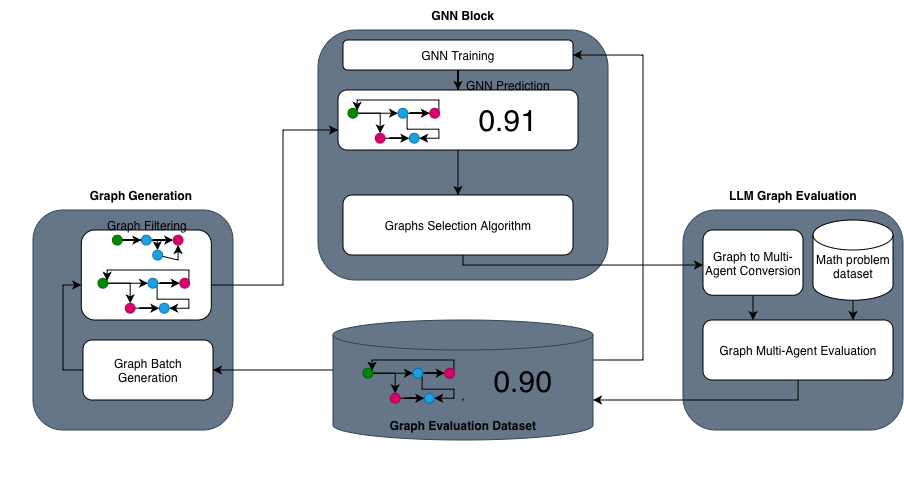
\includegraphics[width=0.75\textwidth]{MLG-project-pipeline.png}
    }
    \caption{Schematic representation of pipeline.}
    \label{fig:pipeline}
\end{figure}

\paragraph{Graph Evaluation Dataset}

The \textit{Graph Evaluation Dataset} serves as the central knowledge repository, storing pairs of graph structures and their corresponding performance evaluations. Each entry consists of a graph \(G \), paired with its empirically measured performance \(p \in \mathbb{R}\). This dataset provides training data \(\{(G_i, p_i)\}_{i=1}^{N}\) for the GNN model and grows iteratively as new evaluations are completed.

\paragraph{Graph Generation Block}

The \textit{Graph Generation Block} produces candidate multi-agent topologies for evaluation. It takes the current \textit{Graph Evaluation Dataset} as input and outputs a batch of \(K\) candidate graph structures. Initially, graphs are sampled randomly from a constrained space. As the dataset grows, the generator transitions to informed sampling strategies including similarity-based generation from top-performing graphs,
using graph similarity algorithms \cite{dwivedi2020algorithmsexactapproximateerrortolerant, JMLR:v12:shervashidze11a, wang2021comprehensivesurveyexperimentalcomparison}.

\paragraph{GNN Block}

The \textit{GNN Block} functions as a surrogate model that predicts multi-agent system performance without requiring costly LLM evaluations. It takes as input the \textit{Graph Evaluation Dataset} \(\{(G_i, p_i)\}_{i=1}^{N}\) for training and \(K\) unevaluated candidate graphs from the generation block. It outputs a trained GNN model \(f_{\theta}: \mathcal{G} \rightarrow \mathbb{R}\), predicted performance values \(\{\hat{p}_1, \ldots, \hat{p}_K\}\), and a filtered subset of top-\(M\) graphs (typically \(M \ll K\)). The task is therefore graph prediction.

The choice of GNN architecture is motivated by the strong dependency between agent interactions and their local neighborhood properties. In multi-agent reasoning systems, an agent's contribution depends critically on the types and features of agents it communicates with. We will primarily 
focus on two attention-based architectures: Graph Attention Networks (GAT) \cite{vel} and Heterogeneous Graph Attention Networks (HetGAT) \cite{wang2021heterogeneousgraphattentionnetwork}. 

For comparison, we also evaluate simpler baseline models including Graph Convolutional Networks (GCN) \cite{kipf2017semisupervisedclassificationgraphconvolutional}, which perform uniform neighborhood averaging, and GraphSAGE \cite{hamilton2018inductiverepresentationlearninglarge}, which uses sampling-based aggregation. These baselines allow us to quantify the benefit of attention mechanisms for this problem domain.

\paragraph{LLM Graph Evaluation Block}

The \textit{LLM Graph Evaluation Block} performs empirical evaluation of selected multi-agent structures on mathematical reasoning tasks. It takes as input the top-\(M\) candidate graphs from the GNN Block and a fixed problem set \(\mathcal{P} = \{(q_1, a_1), \ldots, (q_T, a_T)\}\) from our Math problem dataset. It outputs performance scores \(\{p_j\}\) and new graph-performance pairs \(\{(G_j, p_j)\}_{j=1}^{M}\) that are appended to the Graph Evaluation Dataset.

The evaluation infrastructure is implemented in Python using LangGraph \cite{langgraph2024} for multi-agent orchestration and open-source LLM models. To establish performance baselines, we compare our learned multi-agent topologies against classical single-agent prompting strategies including Chain-of-Thought reasoning \cite{wei2023chainofthoughtpromptingelicitsreasoning}, Self-Consistency \cite{wang2022selfconsistency}, Reflection \cite{shinn2023reflexion}, and Tree-of-Thoughts \cite{yao2023tree}. 

\section{Hypotheses}

We formulate three core hypotheses to guide our experimental investigation:

\textbf{H1} As the Graph Evaluation Dataset expands through iterative evaluations, the GNN surrogate model's predictive accuracy will monotonically improve. We will track correlation metric between predicted and actual performance scores to quantify this improvement over successive iterations.

\textbf{H2} Different base LLM models (e.g., GPT-4, Claude, Llama) and LLM type of agent configurations will yield distinct optimal multi-agent graph structures.

\textbf{H3} As the GNN improves, it will preferentially select high-performing candidates for evaluation, leading to over-representation of successful topologies in the dataset. This bias will cause the model to overestimate performance of new candidates, resulting in disappointing empirical evaluations. This negative feedback naturally re-calibrates the GNN, creating a self-correcting mechanism.

\bibliographystyle{plain}
\bibliography{references}

\end{document}